% !TeX root = ../main.tex
% Add the above to each chapter to make compiling the PDF easier in some editors.

\chapter{Background}\label{chapter:background}
This chapter provides background information on topics which are essential for the understanding of the work presented in this thesis. First, an overview of hard real-time systems and their classification is presented, additionally examining the basics of scheduling techniques used in these systems. Then, an introduction into Dynamic Power Management methods is given, explaining their overall functionality and providing references to related research into the respective subdomains. The concept of genetic algorithms is introduced and the GMPT algorithm, upon which the experiments of this thesis are based on, is illustrated. Finally, boxplots are explained and advice on how to interpret the data displayed by them is provided since they are used throughout this thesis to illustrate experimental results.
\section{Hard Real-Time Scheduling}
Real-time systems constitute a subset of hardware and software systems in which their correctness does not only depend on the precision of the results but also on the time frame within which these results are produced \cite{Ahmed2011}. These systems can further be classified into soft real-time systems, where, in the worst case scenario, missed deadlines may result in a degraded quality of service, and hard real-time systems, where all deadlines must be met constantly to avoid catastrophic failure such as loss of human life. Due to these constraints hard real-time systems are often found in safety-critical applications which frequently prompt the employment of particular scheduling approaches.\\
\hspace*{0.5ex}\hspace{0.5ex} Many common operating systems use dynamic scheduling algorithms where task priorities are determined at runtime. With this approach parameters such as task arrival and execution times don't need to be entirely predictable and the inherent flexibility of such methods allows for better CPU usage, resulting in increased performance. These properties may justify the implementation of dynamic scheduling algorithms in soft real-time systems, however, the schedulability analysis, which would be required for hard real-time systems, is an NP-hard problem making the implementation and verification of such algorithms extremely difficult \cite{Baruah}. Consequently, hard real-time systems often resort to static scheduling methods \cite{Cheng1987}. These trade the potential performance gain and flexibility for a deterministic schedule which facilitates their realization. Since the arrival of tasks and their worst-case execution times (WCET) are usually known beforehand for hard real-time systems, a static, deterministic schedule can easily be calculated. This ultimately yields a series of consecutive time slots, each of which have exactly one task assigned to them. This series can then be executed by the hard real-time system in a cyclic fashion without any task missing its deadline.
\section{Dynamic Thermal Management}
In 1965 Gordon Earle Moore, the co-founder of Intel, hypothesized that for the next decade the number of components on an integrated circuit would double every year \cite{Moore1965}. This hypothesis was revised in 1975 by Moore himself to a doubling of components every 2 years \cite{Moore}. The future of this prediction, also known as Moore's Law, is a hotly debated topic today  and while it has been remarkably accurate in the past, this progress has come with major challenges \cite{Theis2017,Mack2015}. The high number of transistors present in a modern CPU combined with the high frequency at which they operate cause a thermal load on the processor \cite{Mutapcic2009}, which, if left unchecked, can severely damage the CPU and other components affected by the heat dissipation. Furthermore, even if immediate damage may be avoided, high temperatures can have an adverse effect on the lifespan of the processor \cite{Xiang2010,Srinivasan2004} which is a significant concern for embedded real-time systems as they frequently run on the same hardware for decades (eg. automobiles and airplanes).\\
\hspace*{0.5ex}\hspace{0.5ex} To alleviate the problems arising from high CPU thermal loads, hardware cooling devices are commonly employed. However, depending on their application area, their physical size and, to some extend, their cost can make them an inconvenient solution for processor overheating. Another available option (which is often used in conjunction with hardware cooling devices) is Dynamic Thermal Management. This method can be implemented purely as a software component as it tries to control the thermal load by throttling the processor accordingly. To achieve this, one of the following two approaches is taken \cite{Brooks}.
\subsection{Dynamic Power Management}
If Dynamic Power Management (DPM) is employed, the CPU is transitioned between a running and sleep state. When the processor is in the sleep state its power consumption is much lower than when in an active running state. Consequently, the generated heat while in sleep mode is also diminished, giving the processor a chance to partly recover from the high temperatures reached in the running state. The challenge when using this approach is to define suitable criteria which decide when a switch between the two states should happen. The goal for these criteria is to find a satisfactory balance between peak temperature minimization and preserving performance while taking into account factors such as the time it takes to physically switch between the states, the different environments which may affect the thermal behavior of the platform and, in the case of hard real-time systems, the requirement to meet all deadlines. \autoref{fig:i_sched_dpm} shows two exemplary applications of Dynamic Power Management on a series of jobs and Figure 2.2 demonstrates their effect on the CPU temperature (these examples are of pure conceptual nature and not based on any specific algorithm).\\
\begin{figure}[htpb]
  \centering
  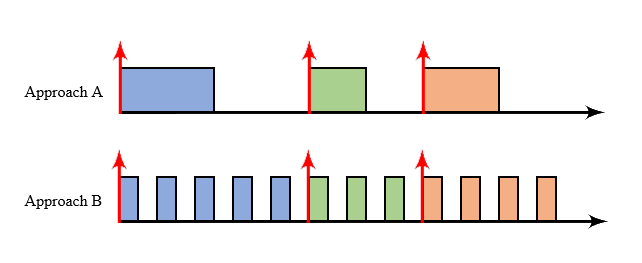
\includegraphics[height=5cm]{figures/dpm_sched}
  \caption[DPM Schedules]{Two Dynamic Power Management Approaches}\label{fig:i_sched_dpm}
\end{figure}
\begin{figure}[htpb]
  \centering

  \pgfplotstableset{col sep=&, row sep=\\}
  % This should probably go into a file in data/
  \pgfplotstableread{
    a & b    \\
    0 & 0 \\
    3 & 3 \\
    5 & 4 \\
    10 & 3 \\
    11.5 & 4.3 \\
    13 & 5 \\
    16 & 4 \\
    18 & 5 \\
    20 & 5.5 \\
    23 & 4.5 \\
  }\exampleA
  \pgfplotstableread{
    a & b    \\
    0 & 0 \\
    1 & 0.8 \\
    2 & 0.7 \\
    3 & 2 \\
    4 & 1.9 \\
    5 & 3 \\
    6 & 2.9 \\
    7 & 3.4 \\
    8 & 3.2 \\
    9 & 3.75 \\
    10 & 3.5 \\
    11 & 4 \\
    12 & 3.75 \\
    13 & 4.25 \\
    14 & 4 \\
    15 & 4.5 \\
    16 & 4.25 \\
    17 & 4.65 \\
    18 & 4.5 \\
    19 & 4.8 \\
    20 & 4.6 \\
    21 & 4.9 \\
    22 & 4.7 \\
    23 & 4.9 \\
  }\exampleB
  % This should probably go into a file in figures/
  \begin{tikzpicture}
    \begin{axis}[
        ymin=0,
        legend style={legend pos=south east},
        grid,
        thick,
        ylabel=Temperature,
        xlabel=Time,
        yticklabels={,,},
        xticklabels={,,}
      ]
      \addplot table[x=a, y=b]{\exampleA};
      \addlegendentry{Approach A};
      \addplot table[x=a, y=b]{\exampleB};
      \addlegendentry{Approach B};
    \end{axis}
  \end{tikzpicture}
  \caption[DPM Temperature Development]{Temperature Development for Approach A and B}\label{fig:i_dpm}
\end{figure}
\subsubsection{Related Work}
Extensive research has been conducted on the Dynamic Power Management approach and its possible use cases. Kumar et al. \cite{Kumar2011} investigates stop-go scheduling deriving a method called JUst Sufficient Throttling (JUST) which is able to minimize the peak temperature of the system, considering a given makespan constraint. Kumar et al. \cite{ACMSpecialInterestGrouponDesignAutomation.2011} furthermore studied shapers as a combination of online and offline calculations to dynamically insert idle times during execution minimizing peak temperature while guaranteeing that all jobs meet their deadlines. Cheng et al. \cite{Cheng2015} propose the Periodic Thermal Management (PTM) method to minimize the peak temperature while satisfying hard real-time constraints. Two models, serving as a trade-off between accuracy and complexity, are derived to calculate the schedule.  Meisner et al. \cite{Meisner} introduce a Dynamic Power Management approach called PowerNap which is used to switch servers into a sleep state when idle, therefore reducing power dissipation.
\subsection{Dynamic Voltage and Frequency Scaling}
As an alternative to Dynamic Power Management it may also be possible to employ Dynamic Voltage and Frequency Scaling (DVFS). Instead of simply switching between sleep and active states, Dynamic Frequency and Voltage Scaling additionally allows to switch between various different active states. In each of these active states the CPU will run at a different frequency and/or voltage level (exemplary illustration in Figure 2.3, not based on any specific algorithm). This allows for the CPU to be tuned more subtly and offering more accurate control over power dissipation and thermal load. While the flexibility of this approach does provide an advantage over the Dynamic Power Management method it also comes with greater complexity, making its implementation more challenging. Compared to the binary state switch performed under DPM a more complicated model is required to derive appropriate schedules, especially when such a schedule is constrained by strict requirements as it is the case in hard real-time systems.\\
\hspace*{0.5ex}\hspace{0.5ex} One common way to access this functionality is via the operating system's kernel which is used as an interface to an available driver (the CPUFreq driver). The CPUFreq driver is ultimately in charge of the frequency and voltage settings and determines what options the kernel will be able to provide. The actual policy according to which the Dynamic Voltage and Frequency Scaling is performed can be set by choosing a CPUFreq governor. The widely adopted Linux kernel implements the following governors \cite{Brodowski}:
\begin{itemize}
\item \textbf{performance:} This governor runs the CPU at the maximum static frequency within preset limits. The only chance for the processor to cool down under this policy are the idle times. While these idle times may be more prevalent than when using other governors due to the higher execution speed, ensuring a low temperature is not the primary concern of this policy.
\item \textbf{powersave:} This governor sets the CPU to the lowest frequency within preset limits. This may extend the execution time of all running jobs, minimizing idle times, but due to this low frequency the power dissipation and the resulting thermal load during active running states is also diminished. From a temperature minimization standpoint, this may sound like a good idea, however, the low execution speed implicates bad performance.
\item \textbf{conservative:} This governor tries to adapt the frequency setting according to the current load on the CPU. It favors low frequencies and once the processor enters an active, executing state it starts to increase the frequency in predefined steps. Once a transition into an idle state is performed, the frequency gets gradually lowered again through the various frequency levels. Therefore, the maximum frequency is only reached if the CPU is under a permanent high load. The precise functionality of this governor can be customized by setting parameters like the granularity of the frequency steps or the threshold for the frequency changes. This improves flexibility and facilitates the use of this policy across a wide range of application fields.
\item \textbf{ondemand:} This governor functions in a similar way to the conservative governor as it also tries to adapt the CPU frequency to the workload, however, it does so more aggressively. As soon as the current workload surpasses a certain threshold the frequency is instantly set to its maximum possible value. Akin to the conservative governor it will gradually decrease the frequency once the CPU is idle. Overall this makes this governor more responsive to sudden high workloads while trading in potential energy efficiency. Like the conservative governor, this policy can also be customized with certain parameters, offering similar flexibility.
\item \textbf{userspace:} This governor provides a more direct control over the frequency setting than the aforementioned policies. When this governor is used, an interface is provided to the root user, with which he can  directly set the frequency to a specific value, as long as the frequency is supported by the given hardware. This allows for the implementation of custom policies in case none of the above satisfy one's needs (even though with considerably more overhead if implemented in the userspace \cite{Pallipadi2006}). 
\end{itemize}
\begin{figure}[H]
  \centering
  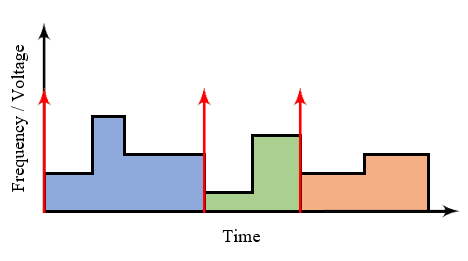
\includegraphics[height=4cm]{figures/dvfs_sched}
  \caption[DVFS Schedules]{Dynamic Frequency and/or Voltage Scaling Approach}\label{fig:i_sched_dvfs}
\end{figure}
\subsubsection{P-States}
A performance state (P-state) is a value pair of a frequency and a voltage defined in the Advanced Configuration and Power Interface (ACPI), an open standard that can be used by operating systems for power management of hardware devices. In the case of processors, P-states are different operating points in which the CPU can function according to different requirements such as performance, power consumption and temperature. The amount and range of available P-states is entirely dependent on the CPU, therefore, certain frequency levels might not be available for dynamic frequency and voltage scaling if the appropriate P-state is not supported by the processor.
\subsubsection{Related Work}
The Dynamic Voltage and Frequency Scaling approach has been widely studied by the scientific community. Sushu et al. \cite{SushuZhang2007} examine the performance optimization of a set of periodic tasks under thermal constraints using DVFS and furthermore proving that this problem is NP-hard. Two algorithms are presented to solve this problem, one pseudo-polynomial optimal approach and one polynomial approximated technique. Chantem et al. \cite{Chantem2009} offer an optimal solution for work maximization considering thermal constraints applicable for general-purpose uniprocessor systems. Additionally the assertion is made that the optimal speed schedule solution must be periodic. Chen et al. \cite{Chen2009} study thermal constrained scheduling for real-time tasks in a DVFS system. Two methods are derived to either minimize response time under a thermal constraint or to minimize the temperature under a timing constraint. Dhiman et al. \cite{Dhiman2007} propose a DVFS technique for multitasking systems which employs an online learning algorithm and the available runtime statistics to determine which voltage and frequency should be used in any given moment. Le Sueur et al. \cite{LeSueur2010} investigates the feasibility of DVFS approaches for modern processors. It is concluded that the effectiveness of voltage and frequency scaling has been reduced in modern systems due to the high static power consumption, smaller dynamic power range and increasingly efficient sleep modes. 
\section{Genetic Algorithm}
Genetic algorithms are an approach to optimization problems based on natural selection \cite{Holland1992}. Much like through evolution in nature, genetic algorithms attempt to improve given solutions to a problem by progressing through several generations of these solutions. At the outset a population of possible solutions (the first generation) is given, large enough in size so that suitable diversity within this population can be ensured. Starting with this population, the genetic algorithm begins iterating over two main steps to recreate the process of natural selection:
\begin{enumerate}
\item \textbf{Selection:} In this first step the current population of solutions is evaluated according to a fitness function. This function serves as a criteria to judge the quality of every individual in the current generation. Based on this fitness, a subset of individuals is chosen as the basis for the next generation. Less fit individuals may also be included in a future generation in order to keep high diversity and avoid premature convergence toward a mediocre solution \cite{Kumar2010}.
\item \textbf{Reproduction:} Based on the individuals selected during the first phase, these solutions are now designated parents which serve as the foundation for the new generation of solutions. The new child individuals are created through combinations of their parent's properties and potential mutation of some of their features.
\end{enumerate}
This procedure is designed to edge ever closer to the optimal solution by picking individuals which are near the optimum. This is done until a termination criteria, such as a satisfactory individual or plateauing of fitness, is met.\\
\hspace*{0.5ex}\hspace{0.5ex} Genetic algorithms are commonly employed in situations where a clear solution to a problem is unknown and not easily derivable. Problems with a high number of unknown variables lend themselves particularly well to this approach since  mathematical solutions to such problems can be very difficult to find, whereas genetic algorithms seemingly find solutions "on their own" by trial and error.
\subsection{GMPT}\label{gmpt}
The elemental features of genetic algorithms such as the large population size and the many iterative developments of each individual make it highly impractical to evaluate the performance of every solution experimentally. This calls for a model which can be used to approximate the fitness of each individual. GMPT resorts to a thermal model that is commonly employed in related research \cite{,Chaturvedi2010,Mohaqeqi2014,Kumar2011}. Here the temperature development of the CPU over time is described by
\begin{equation} \label{eq:model}
T(t)=\frac{A_m}{B_m}+(T(t_0)-\frac{A_m}{B_m})\, e^{-B_m(t-t_0)},
\end{equation}
with $T(t_0)$ being the initial processor temperature and $A_m$ and $B_m$ being factors which describe the CPU peak temperature given by $T^\infty_m=\frac{A_m}{B_m}$, i.e. the temperature $T(t)$ reached for $t \rightarrow \infty$. $A_m$ and $B_m$ are derived from the processor's power consumption (leakage and dynamic) and therefore determine the thermal behavior of the platform for a specific operating mode. Consequently every CPU operating mode has exactly one constant $T^\infty_m$ associated with them.\\
\hspace*{0.5ex}\hspace{0.5ex} While this equation will be used for the evaluation of the experiments, it cannot directly be applied to schedules which run multiple different frequencies. Therefore an additional transformation is performed by using $$T^{PTM}_{peak}(q)=max(T^{st}_1,\,...\,, T^{st}_i,\,...\,, T^{st}_q).$$ The Periodic Thermal Management (PTM) schedule that is returned for each individual by GMPT consists of a period partitioned into various segments, each of which have their own frequency/voltage level assigned to them. By running this schedule, the CPU will eventually reach a state where the temperature at the end of a segment won't change from one period to the next anymore (see \autoref{fig:i_gmpt}). This temperature is designated as the steady temperature $T^{st}_i$. $T^{PTM}_{peak}(q)$ is therefore an upper bound for the temperature which is dictated by the highest frequency/voltage setting within a schedule. This temperature limit is ultimately used to assess the fitness of every schedule via $$fitness=\frac{1}{T^{PTM}_{peak}(q)}.$$ On the basis of this $fitness$ value, individuals are selected and used to generate new schedules. If these new individuals still fulfill the hard real-time constraints they are used as part of the next generation of schedules.
\begin{figure}[H]
  \centering
  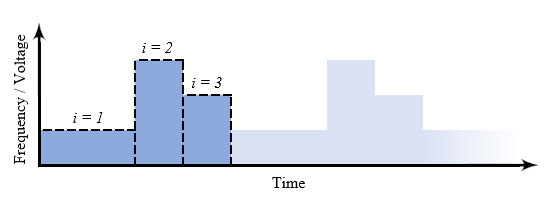
\includegraphics[height=4cm]{figures/gmpt_sched}
  \caption[GMPT Schedule]{One possible PTM schedule for $q = 3$}\label{fig:i_sched_gmpt}
\end{figure}
\begin{figure}[H]
  \centering

  \pgfplotstableset{col sep=&, row sep=\\}
  % This should probably go into a file in data/
  \pgfplotstableread{
    a & b    \\
    0 & 0 \\
    2 & 2 \\
    3 & 6 \\
    4 & 8 \\
    6 & 9.5 \\
    7 & 13 \\
    8 & 15 \\
    10 & 16 \\
    11 & 18 \\
    12 & 19 \\
    14 & 19.5 \\
    15 & 20.5 \\
    16 & 21 \\
    18 & 21 \\
    19 & 21.8 \\
    20 & 22 \\
    22 & 21.5 \\
    23 & 22 \\
    24 & 22 \\
    26 & 21.5 \\
    27 & 22 \\
    28 & 22 \\
    30 & 21.5 \\
    31 & 22 \\
  }\exampleA
  \pgfplotstableread{
    a & b    \\
    0 & 22 \\
    31 & 22 \\
  }\exampleB
  \pgfplotstableread{
    a & b    \\
    0 & 21.5 \\
    31 & 21.5 \\
  }\exampleC
  % This should probably go into a file in figures/
  \begin{tikzpicture}
    \begin{axis}[
        ymin=0,
        legend style={legend pos=south east},
        legend cell align={left},
        grid,
        thick,
        ylabel=Temperature,
        xlabel=Time,
        yticklabels={,,},
        xticklabels={,,}
      ]
      \addplot [red, dashed] table[x=a, y=b]{\exampleB};
      \addlegendentry{$T^{st}_2=T^{st}_3$};
      \addplot [orange, dashed] table[x=a, y=b]{\exampleC};
      \addlegendentry{$T^{st}_1$};
      \addplot [blue] table[x=a, y=b]{\exampleA};
    \end{axis}
  \end{tikzpicture}
  \caption[GMPT Temperature Development]{Possible temperature development for schedule depicted in \autoref{fig:i_sched_gmpt}}\label{fig:i_gmpt}
\end{figure}
\subsection{Boxplots}
Boxplots are a graphical representation of groups of numerical data. A boxplot consists of a box which symbolizes the central 50\% of the data points, the distance between the lower and upper bound of this box is also known as the interquartile range (IQR). Within this box a line marks the median of the entire dataset. Extending out from the upper and lower bound of the box are the so called whiskers. These whiskers extend to the data points furthest away from the box up to a maximum length of 1.5x IQR (based on Tukey boxplot). All data points which lie further away are considered outliers.\\
\hspace*{0.5ex}\hspace{0.5ex} The actual values of the measured parameters in this thesis are not known, but the the measured data points are expected to be distributed normally (or at least closely resemble such a distribution). In this case the 1.5x IQR limit represents the range of values within which 99\% of all measurements are expected to lie.\\
\hspace*{0.5ex}\hspace{0.5ex} Boxplots lend themselves especially well to display the kind of experimental data that has been recorded during this thesis. They can give a simple but clear overview of how the recorded data is distributed an provide a strong indication of where the true value of the measured parameter lies.